% Metódy inžinierskej práce

\documentclass[10pt,slovak,a4paper]{article}

\usepackage[slovak]{babel}
%\usepackage[T1]{fontenc}
\usepackage[IL2]{fontenc} % lepšia sadzba písmena Ľ než v T1
\usepackage[utf8]{inputenc}
\usepackage{graphicx}
\usepackage{url} % príkaz \url na formátovanie URL
\usepackage{hyperref} % odkazy v texte budú aktívne (pri niektorých triedach dokumentov spôsobuje posun textu)

\usepackage{cite}
\usepackage{float}
%\usepackage{times}

\pagestyle{headings}

\title{Techniky spracovanie veľkých dát\thanks{Semestrálny projekt v predmete Metódy inžinierskej práce, ak. rok 2023/24, vedenie: Vladimír Mlynarovič}} % meno a priezvisko vyučujúceho na cvičeniach

\author{Tomáš Zenka\\[2pt]
	{\small Slovenská technická univerzita v Bratislave}\\
	{\small Fakulta informatiky a informačných technológií}\\
	{\small \texttt{xzenka@stuba.sk}}
	}

\date{\small 5. november 2023} % upravte



\begin{document}

\maketitle

\begin{abstract}
Článok skúma a porovnáva techniky spracovania veľkého množstva dát, čo je kľúčové v dnešnej digitálnej dobe, kde sa generuje obrovské množstvo informácií. Cieľom je poskytnúť prehľad o moderných prístupoch a nástrojoch určených na manipuláciu s masívnymi dátovými súbormi. Tieto nástroje zahŕňajú distribuované systémy na spracovanie dát, algoritmy strojového učenia a metriky na hodnotenie kvality dát. Dôraz sa kladie na potrebu rýchleho spracovania dát v reálnom čase, čo umožňuje rýchlu analýzu a tvorbu hodnotných poznatkov z týchto objemných dátových zdrojov. Článok taktiež uvádza príklady aplikácií v rôznych odvetviach, ako je medicína, finančníctvo a priemysel. Spracovanie veľkého množstva dát sa stáva nevyhnutným nástrojom pre konkurencieschopnosť a inovácie v súčasnom digitálnom prostredí.
\end{abstract}
\newpage


\section{Úvod}

Pojem "veľké dáta" (Big Data) odkazuje na súbor dát, ktorých veľkosť, komplexnosť a rýchlosť rastu je rapídna. Preto sú zložité na spracovanie a analýzu.\cite{ZakladneInfo} Cieľom článku je poskytnúť prehľad o prístupoch a technikách na manipuláciu s týmito dátami. Tieto nástroje zahŕňajú distrubuované systémy na spracovanie dát~\ref{Distribuovane}  a metriky na hodnotenie kvality dát~\ref{Metriky}. Článok sa zameriava aj na rýchle spracovanie dát v reálnom čase~\ref{RychleSpracovanie}. Na záver sú uvedené aplikácie v rôznych odvetviach~\ref{Aplikacie}.



\section{Techniky spracovania veľkého množstva dát} \label{Techniky}

Rýchle tempo digitalizácie vytvára obrovské množstvo dát. V dnešnej digitálnej dobe je dôležitá výzva spracovanie veľkého množstva dát. Len za posledné desaťročia sa celkový počet dát na svete zvýšil na 1,8 ZB\cite{Survey}. Preto boli na tieto účely spracovanie týchto dát vyvinuté rôzne techniky a nástroje. Umožňujú používateľovi efektívne manipulovať a pracovať s masívnymi dátovými súbormi.

\paragraph{Historické súvislosti.}
Pri pochopení spracovania veľkých dát pomáha pochopiť aj to ako sa vyvíjali techniky spracovania dát od počiatkov až po súčastnosť. Ako sme prešli od kompletne mechanických zariadení, cez moderné výpočtové technológie, až po súčastné technológie na spracovanie veľkých dát.

\subsection{Distribuované systémy na spracovanie dát} \label{Distribuovane}

Distribuované systémy na spracovanie dát predstavujú kľúčový prvok v digitálnom svete. Rýchlosť a škálovateľnosť sú najdôležitejšie aspekty. Rozoberieme si základné systémy, ktoré umožňujú rýchlo a efektívne získavať relevantné informácie z masívnych dátových sád.

\subsubsection {Hadoop: MapReduce}

Hadoop je programovací framework (rámec) na podporu spracovania veľkých dátových súborov. Bol vyvinútý spoločnosťou Google MapReduce. V súčastnosti sa v praxi používa Appache Hadoop, ktorý sa rozdeľuje na rôzne časti:

\begin{enumerate}
\item Hadoop Kernel
\item MapReduce
\item HDFS
\end{enumerate}

Hlavnou výhodou frameworku Hadoop je úložný systém odolný voči chýbam s názvom Hadoop Distributed File System (HDFS). HDFS rozdeluje systém súborov do 128 MB blokov~\cite{HDFS}. Na obrázku~\ref{HadoopObrazok} je vykreslená architektúra HDFS. Je schopný uložiť obrovské množstvo informácií, postupne sa škálovať a to najdôležitej je, že dokáže prežiť zlyhanie významných častí infraštruktúry úložsika.
\begin{figure}[H]
  \centering
  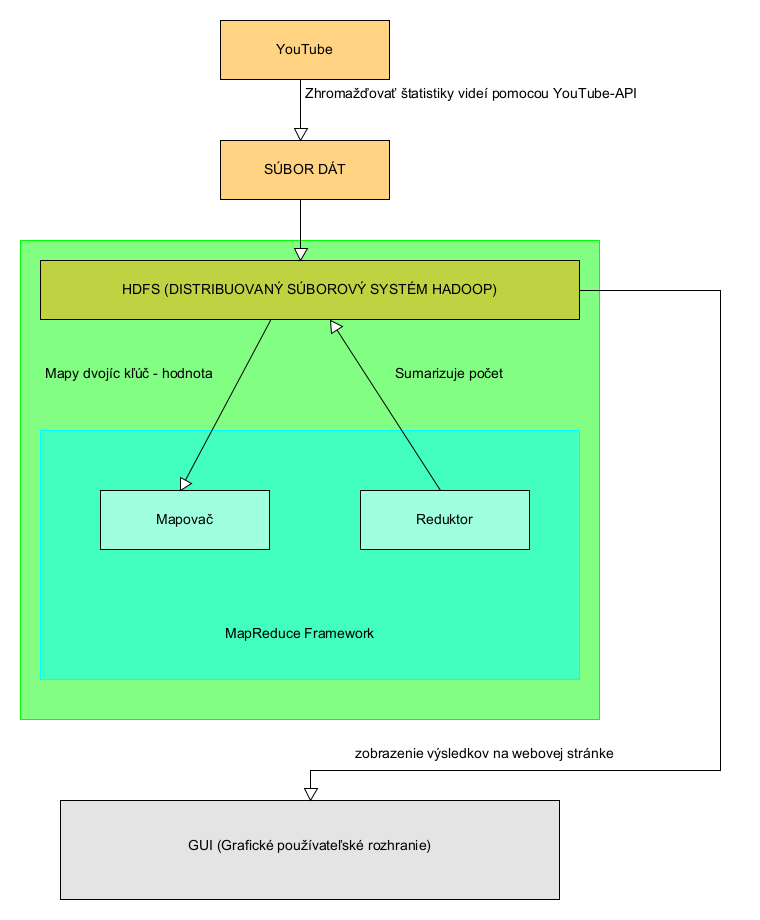
\includegraphics[width=1\textwidth]{HDFS_prelozene.png}
  \caption{Architektura HDFS, spracované podľa \cite{HadoopObrazok}}
  \label{HadoopObrazok}
\end{figure}

Hadoop vytvára zhluky strojov a koordinuje prácu medzi nimi. Ak jeden zlyhá tak Hadoop pokračuje bez stráty. Prácu zlyhaného článku prehodí na zvyšné počítače.

Hlavnou zložkou ekosystému Hadoop je MapReducce framework. Umožňuje rozdelenie problému a dát na menšie a spustiť ich paralelne. MapReduce má dve funkcie:

\begin{itemize}
\item map - ako vstup hodnota/klúč páru a generuje intemediate set párov klúčov/hodnôt
\item reduce - spája intermediate set hodnôt s rovnakým intermediate set klúčov
\end{itemize}
\cite{ZakladneInfo}

\subsubsection {Apache Spark}

Apache Spark je nová generácia systémov na spracovanie veľkých dát. Systém Apache Spark pozostáva z hlavných systémov:
\begin{itemize}
\item Spark core (jadro)
\item Upper-level libraries
\end{itemize}
V porovnaní s Hadoop MapReduce je Apache Spark rýchlejší a všestranejší. Vďaka knižniciam sa dá použiť na strojové učenie (knižnica Spark’s MLlib), grafická analýza (knižnica GraphX), prúdové spracovanie (knižnica Spark Streaming) a aj na spracovanie štruktúrovaných dát (knižnica Spark SQL). Kombinuje jadro pre distrubuované výpočty s pokročilým programovacím modelom pre spracovanie v pamäti (in-memory processing)~\ref{InMemory}. Zachováva rovnakú možnosť škálovania a odolnosti voči chybám ako Hadoop MapReduce, avšak poskytuje viacstupňový model programovania. Celkovo je rýchlejší a oveľa jednoduchši na používanie.~\cite{Apache}

\subsection {Metriky na hodnotenie kvality dát} \label {Metriky}
Veľké dáta sú novým konceptom a ešte nie je zaužívaný štandart na hodnotenie kvality dát v oblasti veľkých dát. V literatúre nájdeme mnoho rôznych definícii, ale jednu vec majú spoločnú. A to, že kvalita údajov závisí od viacerých vlastností. Predovšetkým od podnikateľského prostredia , ktoré dáta používa. Je veľmi ťažké merať kvalitu údajov vo veľkých dátach. Najčastejšie sa sa používva hirararchický štandard kvality údajov. Sú dimenzie kvality údajov, ktoré sú bežne akceptované a často používané:

\begin{itemize}
\item \emph {Dostupnosť}
	\begin{itemize}
	\item Prístupnosť

	 - úroveň obtiažnosti získavania údajov používateľom, úzko spojená so stupňom otvorenosti údajov, vyšší stupeň otvorenosti znamená vyšší stupeň prístupnosti
	\item Aktuálnosť

	 - časové oneskorenie od generovania a získavania údajov po jeho využitie, pri veľkých dátach sa obsah rýchlo mení, ciže aktuálnosť je veľmi dôležitá
	\item Autorizácia

	 - či jednotlivec má právo používať údaje
	\end{itemize}
\item \emph {Použiteľnosť}
	\begin{itemize}
	\item Dôveryhodnosť

	 - na vyhodnotenie nečíselnýchh údajov, tri faktory: spoľahlivosť zdrojov, normalizácia údajov a čas vytvorenia údajov
	\item Definícia/Dokumentácia

	- špecifikácia údajov zahŕňajúc názov údajov, definíciu, rozsahy platných hodnôt atď.
	\item MetaData

	- popisujú rôzne aspekty súborov údajov, aby znížili problémy nedorozumenia alebo nezrovnalostí
	\end{itemize}
\item \emph {Spoľahlivosť}
	\begin{itemize}
	\item Presnosť

	- na zistenie presnosti hodnoty údajov sa hodnota porovnáva so známou referenčnou hodnotou, v niektorých prípadoch sa presnosť dá ľahko zmerať, ale vo väčšine pripadoch je meranie sťažené, lebo presnosť úzko súvisí s kontextom
	\item Konzistencia

	- či je logický vzťah medzi korelovanými údajmi správny a úplný
	\item Celistvosť

	- odlišné významy na základe kontextu, v databáze musia všetky charakteristiky údajov byť správne, v informatickej bezpečnosti to znamená udržanie a zabezpečenie presnosti a konzistencie údajov, údaje 	nemožno upravovať neoprávneným spôsobom
	\item Úplnosť

	- hodnoty všetkých zložiek jedného údaja sú platné
	\end{itemize}
\item \emph {Relevantnosť}
	\begin{itemize}
	\item Fitness

	- dvojúrovňové požiadavky: množstvo údajov používaných používateľmi, do akej miery vytvorené údaje zodpovedajú potrebám používateľov
	\end{itemize}
\item \emph {Kvalita prezentácie}
	\begin{itemize}
	\item Čitateľnosť

	- schopnosť obsahu údajov byť správne vysvetlená podľa známych alebo dobre definovaných pojmov, atribútov, jednotiek atď.
	\item Štruktúra

	- označuje úroveň náročnosti transformácie neštruktúrovaných alebo pološtruktúrovaných údajov na štruktúrované údaje pomocou technológií 
	\end{itemize}
\end{itemize}

~\cite{Metrics}


\section {Rýchle spracovanie dát v reálnom čase} \label{RychleSpracovanie}

Táto sekcia sa zameriava a kladie dôraz na rýchle a efektívne spracovanie dát v danom čase. V súčastnom digitálnom prostredí sa obzvlásť kladie dôraz na analýzu dát v okamihu kedy sú generované.

\subsection {Spracovanie v pamäti} \label{InMemory}

Spracovanie v pamäti je základom pre Apache Spark. Umožňuje mu to ukladať prechodné dáta do pamäte, čo má za následok to, že namiesto aby všetky dáta išli na disk a neskôr sa vyberali z disku, tak sú uložené dočasne v pamäti kde čakujú na spracovanie. Toto urýchluje celý proces spracovania dát.~\cite{Apache}

V databázach, ktoré používajú in-memory processing sa veľké množstvo dát generuje v reálnom čase. Je potrebné ho v reálnom čase aj spracovať. Väčšina dát prichádza priamo do pamäte na spracovanie, len málo dát ide na pevný disk na dlhodobé uloženie. ~\cite{InMemoryArticle}

\subsection {Systémy na spracovanie tokov}

Jedná sa o klúčové nastroje v prípade ak nám priebežne prúdi veľké množstvo dát. Dokážu ich rýchlo a efektívne spracovať. Takéto dáta môžu byť napríklad dáta zo senzorov alebo zo sociálnych medií.

Momentálne najpoužívanejší sytém je Apache Kafka. Na obrázku ~\ref{ApacheKafkaObrazok} je rozpísaná architektúra Apache Kafka. Výhody Apache Kafka sú, že je škálovatelná a spoľahlivá. ~\cite{ApacheKafka}
\begin{figure}[H]
  \centering
  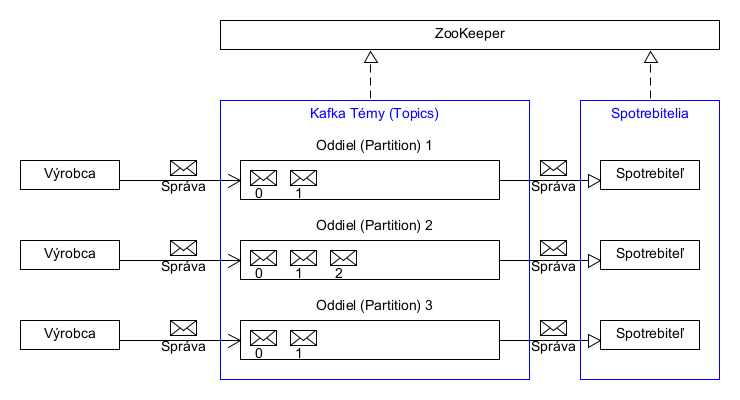
\includegraphics[width=1\textwidth]{Kafka_prelozene.png}
  \caption{Architektura Apache Kafka, spracované podľa \cite{ApacheKafka}}
  \label{ApacheKafkaObrazok}
\end{figure}



\section {Aplikácie v rôznych odvetviach} \label {Aplikacie}

V praxi sa využíva hlavne framework Apache Spark v rôznych odvetviach ako napríklad:
\begin{itemize}
\item Zdravotníctvo \ref{Zdrav}
\item Financie \ref {Fin}
\item Zábavný priemysel \ref {Zabav}
\end{itemize}

\subsection {Zdravotníctvo} \label {Zdrav}

Využíva sa na analýzu zdravotných záznamov pacienta. Pomáha identifikovať či je pacient náchylný ku zdravotným komplikácia v budúcnosti. Taktiež spracováva dáta z genómového sekvenovania (genomic sequencing).

\subsection {Financie} \label {Fin}

Poskytuje aktuálny prehľad, ktorý pomáha pri robení správnych rozhodnutí. Napríklad v oblasti segmentácie zákazníkov, hodnotení úverového rizika alebo pri cielenej reklame.

\subsection {Zábavný priemysel} \label {Zabav}

Hlavne v oblasti videoherného priemyslu pomáha s rozpoznávaním vzorov. Neskôr využité na selektívnu reklamu alebo automatická zmena náročnosti na základe hráčskych schopností.

\cite {ApacheAplication}

\section{Záver} \label{zaver} % prípadne iný variant názvu
Spracovanie veľkého množstva dát sa stalo kľúčovou súčasťou 21. storočia. S narastajúcim objemom dát, ktoré sa podľa predpokladov búdu zdojnásobovať každé dva roky v blízkej budúcnosti\cite{Survey}, sa nástroje na ich spracovanie stávajú povinnosťou pre konkurencieschopnosť a inováciu. Predstavili sme si moderné techniky spracovania veľkých dát, ktoré sú rýchle a efektívne. Taktiež je veľmi dôležité spracovanie v realnom čase. S ohľadom na budúcnosť si myslím, že táto oblasť bude ďalej rásť a rozvíjať sa.


%\acknowledgement{Ak niekomu chcete poďakovať\ldots}


% týmto sa generuje zoznam literatúry z obsahu súboru literatura.bib podľa toho, na čo sa v článku odkazujete
\bibliography{literatura}
\bibliographystyle{plain} % prípadne alpha, abbrv alebo hociktorý iný
\end{document}
